\documentclass{beamer}
\mode<presentation>
{
  \usetheme{Frankfurt}
  \usecolortheme{crane}
  \setbeamertemplate{blocks}[rounded][shadow=true]
  % or ...
  %\setbeamercovered{transparent}
  % or whatever (possibly just delete it)
}
\usepackage{subfigure}
\usepackage{pgf,pgfarrows,pgfshade}
\usepackage[english]{babel}
\input{../cimis_acronyms}

\title[ET0] % (optional, use only with long paper titles)
{California \ac{ET0}}
%\subtitle{}

\author{Quinn Hart}

\institute[CalSpace] % (optional, but mostly needed)
{
  CalSpace \\
  University of California, Davis \\
  qjhart@ucdavis.edu
}

\date[GEO289 W06] % (optional, should be abbreviation of conference name)
{GEO289 W06}

\begin{document}

\titlepage
\section[Overview]{Evapotranspiration Overview}

\subsection{}

\begin{frame}
  \frametitle{Overview}
  \begin{itemize}
  \item Spatially distributed ET0 maps
  \item $(\unit[2]{km})^2$ resolution
  \item \ac{NOAA} \ac{GOES} imager
  \item \ac{CIMIS} weather station data
  \end{itemize}

%  \begin{block}{}
%    The goal of this project is to calculate spatially distributed daily
%    \ac{ET0} and produce daily \ac{ET0} maps for the State of California
%    at high spatial resolution, $(\unit[2]{km})^2$.  The methodology for
%    creating statewide \ac{ET0} maps used \ac{NOAA} \ac{GOES} imager
%    data, combined with the \ac{CIMIS} weather station data and
%    ancillary datasets.
%  \end{block}
\end{frame}

\begin{frame}
  \frametitle{California \ac{ET0} Zones}
  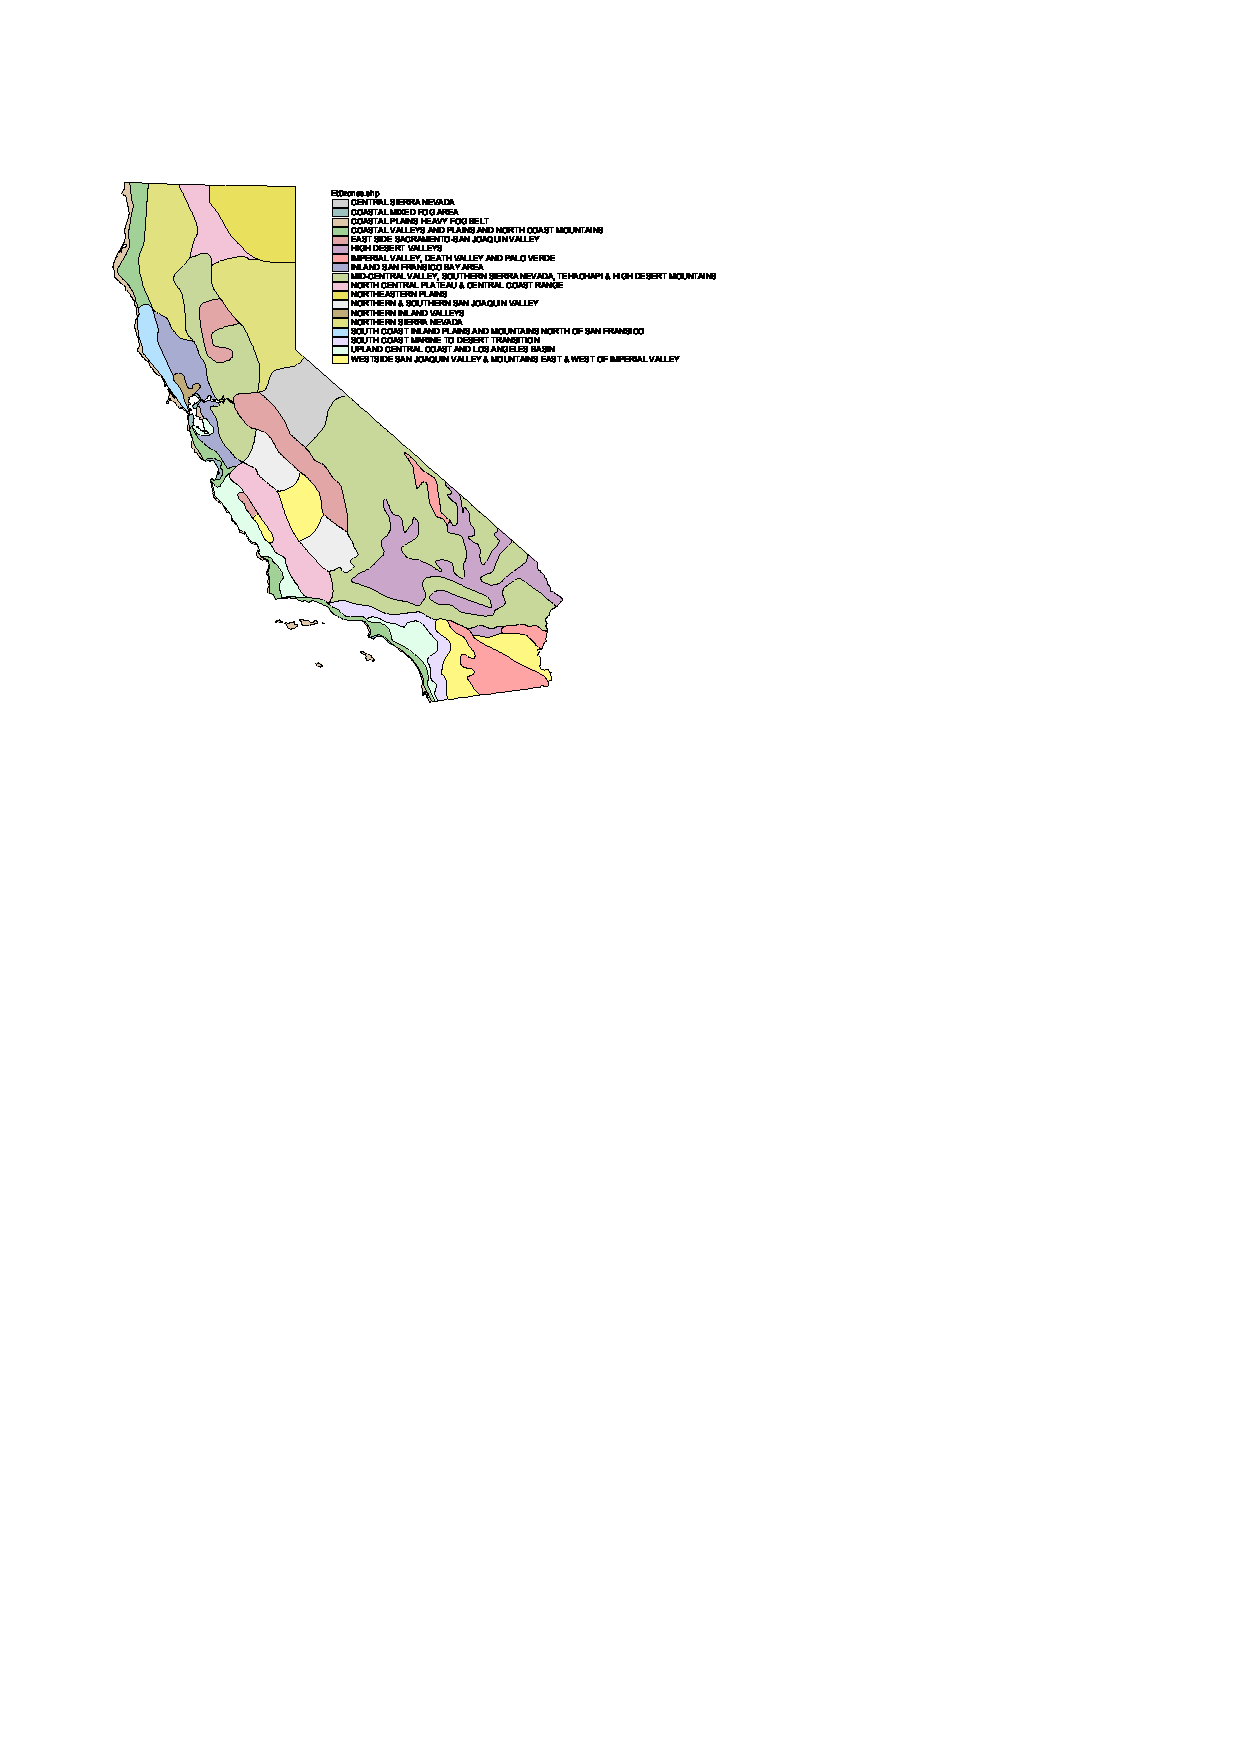
\includegraphics[width=0.8\textwidth]{etomap_simple.pdf}
\end{frame}

\begin{frame}
  \frametitle{CIMIS Stations}
   \begin{columns}
     \column{0.5\textwidth}
     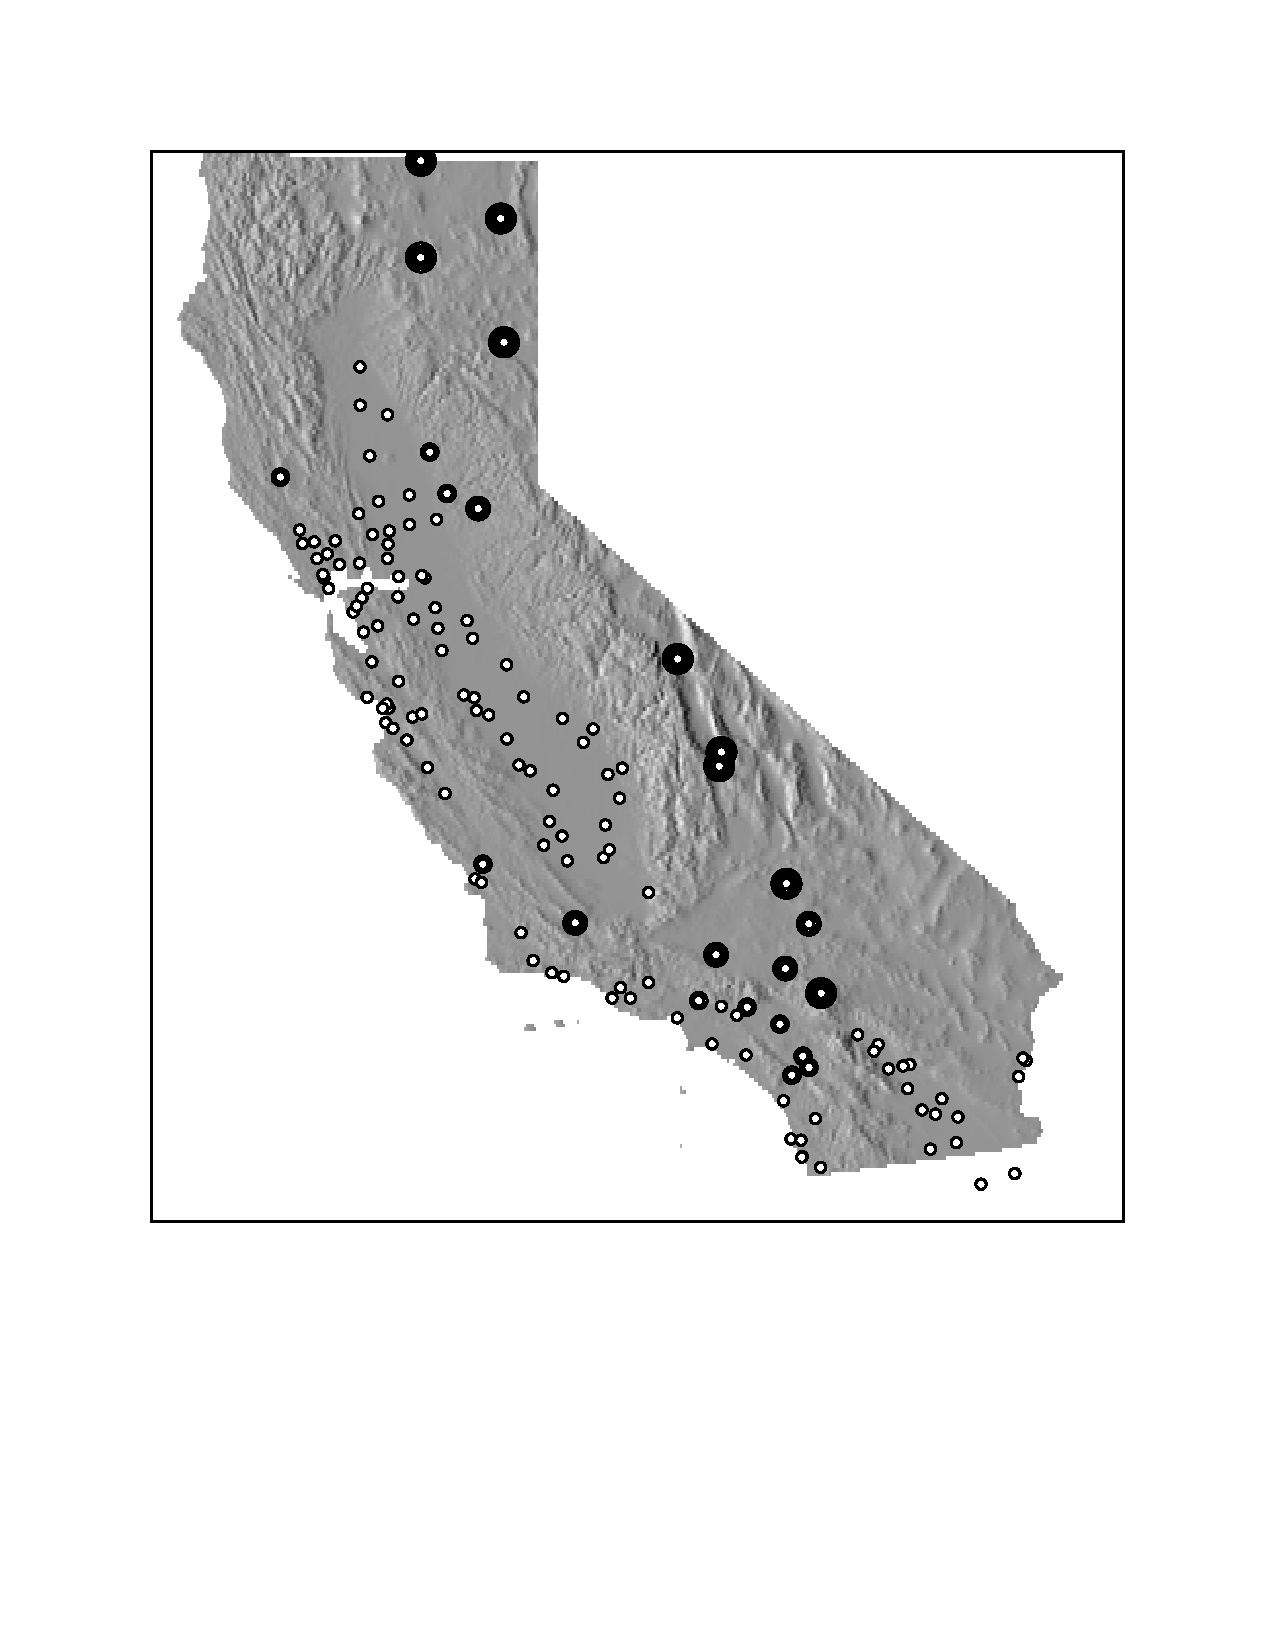
\includegraphics[width=1\textwidth]{stations}
     \column{0.5\textwidth}
     \begin{block}{}
       The \ac{CIMIS} weather stations are located throughout California, but
       with special emphasis on regions with high agricultural use.
       Parts of CA, including mountainous regions, urban and desert
       landscapes are less well covered with representative stations.
     \end{block}
   \end{columns}
  \label{fig:stations}
\end{frame}

% \begin{frame}
% \frametitle{Symbols}
%   \label{tab:symbols}
%   \begin{tabular}{l|l|l}
%     Symbol & Description & Units \\
%     \hline \hline
%     \acs{ET0} & \acl{ET0} & \unitfrac{mm}{day} \\
%     \acs{Tm}  & \acl{Tm}  & \unit{\ensuremath{^\circ}C} \\
%     \acs{Tn}  & \acl{Tn}  & \unit{\ensuremath{^\circ}C} \\
%     \acs{Tx}  & \acl{Tx}  & \unit{\ensuremath{^\circ}C} \\
%     \acs{dewp}  & \acl{dewp}  & \unit{\ensuremath{^\circ}C} \\
%     \acs{U2} & \acl{U2}   & \unitfrac{m}{s} \\    
%     \acs{RHx}& \acl{RHx}  & \unit{\%}\\
%     \acs{ea} & \acl{ea}   & \unit{kPa} \\
%     \acs{es} & \acl{es}   & \unit{kPa} \\
%     \acs{psyc}& \acl{psyc}& \unitfrac{kPa}{\ensuremath{^\circ}C} \\
%     \acs{vp}  & \acl{vp}  & \unitfrac{kPa}{\ensuremath{^\circ}C} \\
%     \acs{Rn} & \acl{Rn} & \unitfrac{MJ}{m\ensuremath{^{2}}\,day} \\
%     \acs{Rnl} & \acl{Rnl} & \unitfrac{MJ}{m\ensuremath{^{2}}\,day} \\
%     \acs{Rs} &  \acl{Rs}   & \unitfrac{MJ}{m\ensuremath{^{2}}\,day} \\
%     \acs{Rso} &  \acl{Rso}   & \unitfrac{MJ}{m\ensuremath{^{2}}\,day} \\
%     \acs{G} & \acl{G}& \unitfrac{MJ}{m\ensuremath{^{2}}\,day} \\
%     \acs{K} &  \acl{K}   & \\
%     \ensuremath{\sigma} & Stefan-Boltzman constant = $4.903e^{-9}$ & \unitfrac{MJ}{m\ensuremath{^2}K\ensuremath{^4}\,day} \\
%     \ensuremath{\alpha} & Albedo & \\
% %%    \acs{em} & \acl{em} & \\
%   \end{tabular}
% \end{frame}

\begin{frame}
  \frametitle{Processing Steps}
  \includegraphics[width=1\textwidth]{et0}
  \label{fig:process}
\end{frame}

\begin{frame}
  \frametitle{Some \ac{ET0} Equations}
  \begin{align*}
    \acs{ET0} &= \frac{0.408  \Delta  (\acs{Rn} - \acs{G}) + \gamma \frac{900}{ \acs{Tm} + 273} \acs{U2} (\acs{es} - \acs{ea})}{\Delta + \gamma  (1 + 0.34 \acs{U2})} \\
    \acs{Rn} &= \acs{Rns} - \acs{Rnl} \\
    \acs{Rns} &= (1 - \alpha) \acs{Rs} \\
    \acs{Rs} &= \acs{K} \acs{Rso}
  \end{align*}
\end{frame}

\begin{frame}
  \frametitle{Technology}
  \begin{itemize}
  \item GRASS
    \begin{itemize}
    \item r.solpos - Solar parameters
    \item s.daymet - Calculate daymet rasters
    \item r.heliosat - Integrated solar energy
    \item 4 minor commands
    \end{itemize}

  \item Make to control flow

  \item GOES Receiver`

  \item CIMIS Downloads

  \end{itemize}
\end{frame}
\section[Rs]{Net Radiation}

\subsection{}

 \begin{frame}
   \frametitle{Clear Sky Insolation} 
   \begin{itemize}
   \item Heliosat-II model
     \begin{itemize}
     \item Linke Turbidity (aerosols,\ac{RHx},$O_3$,Rayleigh)
     \item relates optical depth for general atmos. to Rayleigh
     \item DB of Linke turbidity factor.
     \end{itemize}
   \item Solar Geometry
   \end{itemize}
\end{frame}

\begin{frame}
  \frametitle{Clear Sky Insolation (June)}
  \begin{columns}
    \column{.5\textwidth}
    \begin{block}{ASCE}
      \includegraphics[width=1\textwidth]{2003-06-18/FAO_Rso.png}
    \end{block}
    \column{.5\textwidth}
    \begin{block}{Heliosat-II}
      \includegraphics[width=1\textwidth]{2003-06-18/Rso.png}
    \end{block}
  \end{columns}
\end{frame}

\begin{frame}
  \frametitle{Clear Sky Insolation (December)}
  \begin{columns}
    \column{.5\textwidth}
    \begin{block}{ASCE}
      \includegraphics[width=1\textwidth]{2003-12-21/FAO_Rso.png}
    \end{block}
    \column{.5\textwidth}
    \begin{block}{Heliosat-II}
      \includegraphics[width=1\textwidth]{2003-12-21/Rso.png}
    \end{block}
  \end{columns}
\end{frame}

\begin{frame}
  \frametitle{Cloud Brightness}

   \begin{block}{Hourly Integrations}
   \begin{center}
     \resizebox{0.6\textwidth}{!}{\input{insolation.pdf.tex}}
   \end{center}
   \end{block}


   \begin{itemize}
     
   \item Cloud Brightness $n_i = \frac{V_i - \rho_i}{BX_i - \rho_i}$
     \begin{itemize}
     \item $V_i$ is \ac{GOES} visible
     \item $\rho_i$ is \ac{GOES} visible albedo
       \begin{itemize}
       \item Min. brightness over 2 weeks
       \end{itemize}
     \item $BX_i$ is max pixel brightness
       \begin{itemize}
       \item Max in 9x9 average
       \end{itemize}
     \end{itemize}
   \end{itemize}
\end{frame}

\begin{frame}
  \frametitle{Clear Sky Factor, \acs{K}}
  \begin{itemize}
  \item Clear Sky Factor
    \begin{equation*}
      k_i= \begin{cases}
        1.2 & n_i > 1.2 \\
        n_i & 0.2 < n_i < 1.2 \\
        5n_i^2/3+n_i/3 +1/15 & -0.1 < n_i < 0.2 \\
        0.05 & n_i < -0.1 
      \end{cases}
    \end{equation*}
  \end{itemize}
\end{frame}

\begin{frame}
  \frametitle{Clouds (2006-03-06)}

  \includegraphics[width=0.33\textwidth]{2006-03-06/vis0900.png}
  \includegraphics[width=0.33\textwidth]{2006-03-06/vis1200.png}
  \includegraphics[width=0.33\textwidth]{2006-03-06/vis1500.png}

  \includegraphics[width=0.33\textwidth]{2006-03-06/p0900.png}
  \includegraphics[width=0.33\textwidth]{2006-03-06/p1200.png}
  \includegraphics[width=0.33\textwidth]{2006-03-06/p1500.png}

\end{frame}


\begin{frame}
  \frametitle{Clear Sky Factor}

  \includegraphics[width=0.33\textwidth]{2006-03-06/Rso.png}
  \includegraphics[width=0.33\textwidth]{2006-03-06/K.png}
  \includegraphics[width=0.33\textwidth]{2006-03-06/Rs.png}

\end{frame}

\begin{frame}
  \frametitle{Measured vs. \ac{GOES} Insolation \unitfrac{MJ}{m\ensuremath{^{2}}\,day}}
   \includegraphics{Rs_R.pdf}
\end{frame}

\begin{frame}
  \frametitle{Spatial Distribution of Errors}
  \begin{columns}
    \column{0.5\textwidth}
    \includegraphics[height=0.8\textheight]{sr}
    \column{0.5\textwidth}
    \begin{block}{}
      These data are averaged over all measurements for 18
      months.  The standard error is reported in percent difference
      between the measurements and predictions.    
    \end{block}
  \end{columns}
\end{frame}

\begin{frame}
  \frametitle{Measured vs. Estimated Cloud Cover}
  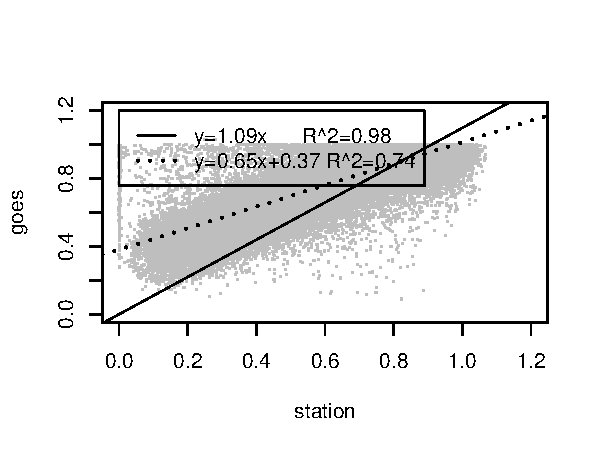
\includegraphics{K_R.pdf}
\end{frame}

\begin{frame}
  \frametitle{Long Wave Radiation \acs{Rnl},\unitfrac{MJ}{m\ensuremath{^{2}}\,day}}
  \begin{equation*}
    \acs{Rnl} = -(1.35K-0.35)(0.34-0.14\sqrt{e_a})\sigma\frac{(T_x+273.16)^4+(T_n+273.16)^4}{2}
  \end{equation*}
  \vspace*{-1cm}
  \includegraphics{Rnl_R.pdf}
\end{frame}


\section[Interpolation]{Parameter Interpolation}
\subsection{}

\begin{frame}
  \frametitle{CIMIS Stations}
   \begin{columns}
     \column{0.5\textwidth}
     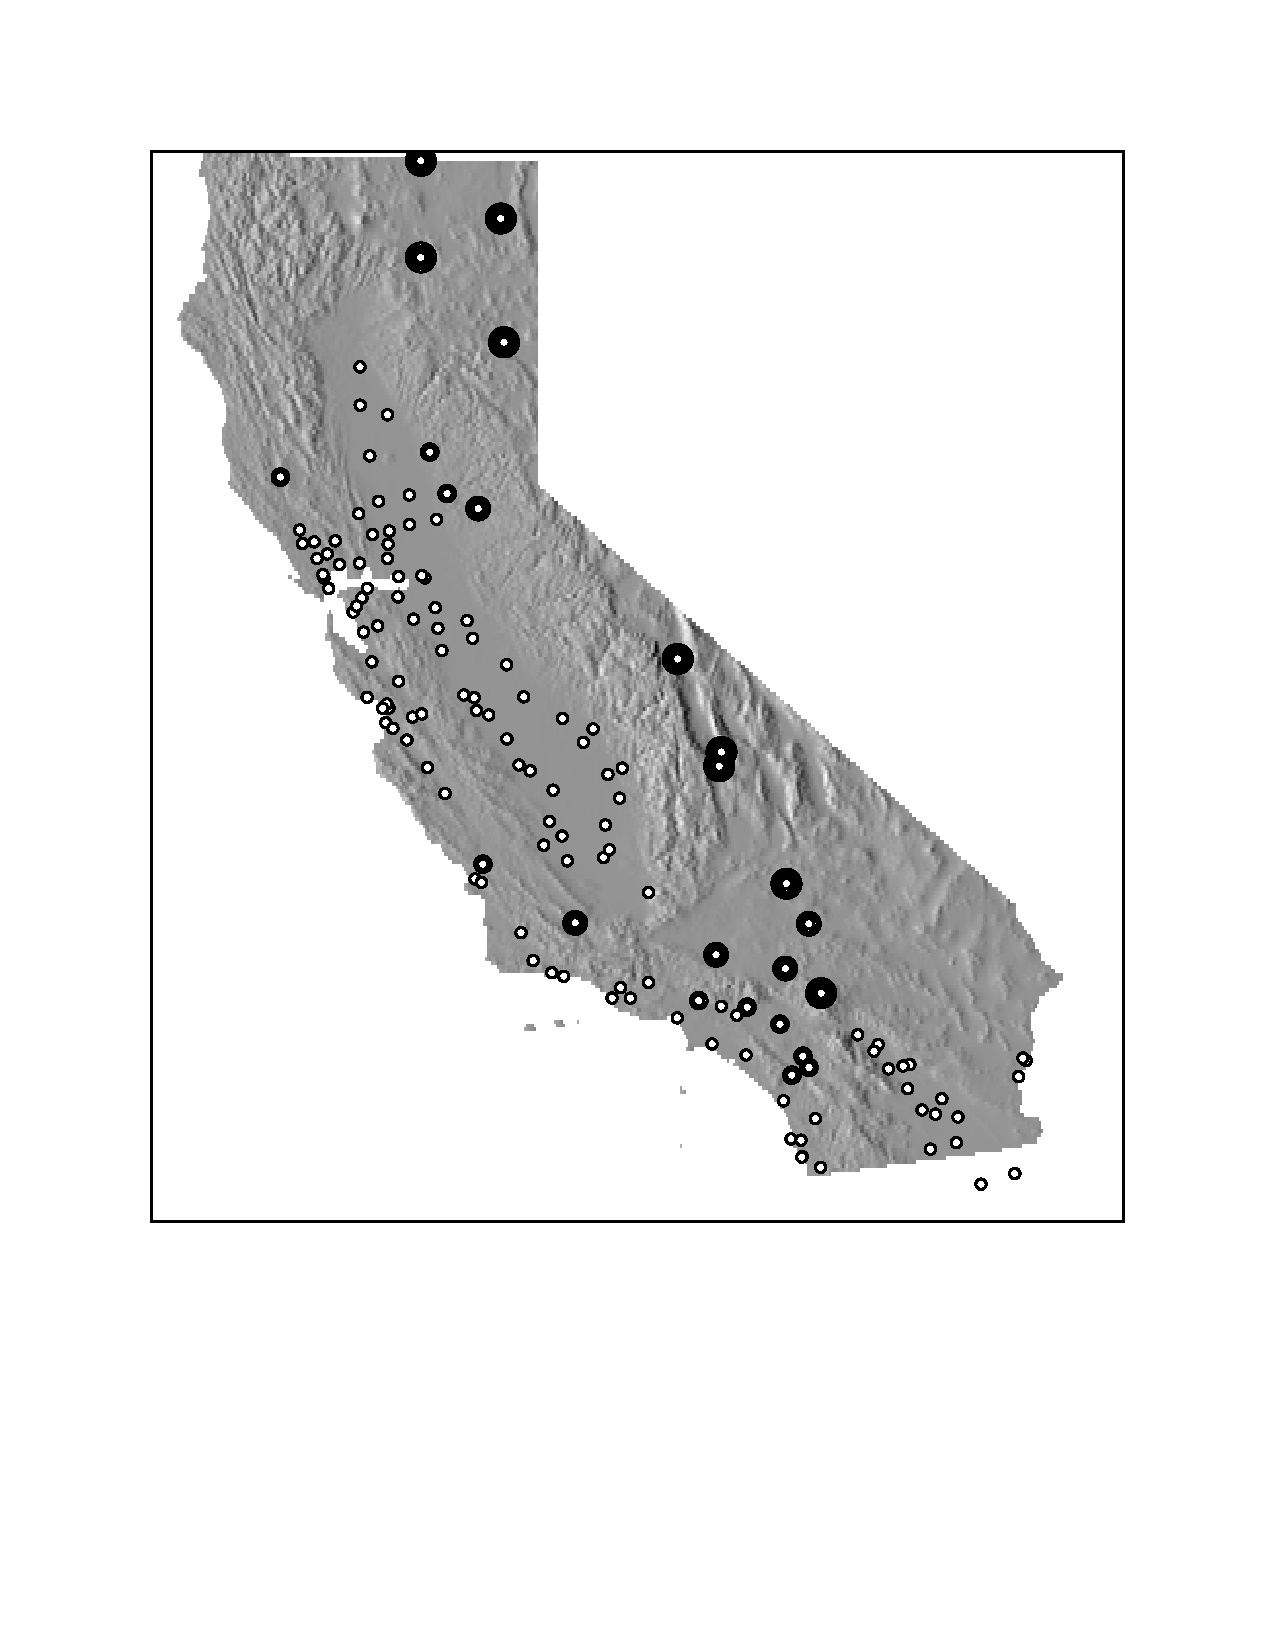
\includegraphics[width=1\textwidth]{stations}
     \column{0.5\textwidth}
     \begin{block}{}
       The \ac{CIMIS} weather stations are located throughout California, but
       with special emphasis on regions with high agricultural use.
       Parts of CA, including mountainous regions, urban and desert
       landscapes are less well covered with representative stations.
     \end{block}
   \end{columns}
\end{frame}

\begin{frame}
  \frametitle{Interpolation Methods}
  \begin{columns}
    \column{.5\textwidth}
    \begin{block}{Daymet}
      \begin{itemize}
      \item Inverse distance methodology (X,Y,Z)
      \item Truncated Gaussian Curves
      \item Two Parameters
        \begin{itemize}
        \item Shape
        \item Truncation Distance
        \end{itemize}
      \item Chosen Daily
      \item Minimize cross-validation
      \end{itemize}
    \end{block}
    \column{.5\textwidth}
    \begin{block}{Splines}
      \begin{itemize}
      \item (X,Y) and (X,Y,Z)
      \item Continuous Derivatives
      \item Three Parameters
        \begin{itemize}
        \item Tension
        \item Smoothing
        \item Scale (Z)
        \end{itemize}
      \item One time estimation
        \begin{itemize}
        \item Minimize Error
        \item Visual inspection
        \end{itemize}
      \end{itemize}
    \end{block}
  \end{columns}
\end{frame}

\begin{frame}
  \frametitle{Temperature}
  \begin{columns}
    \column{.5\textwidth}
    \begin{block}{}
      \begin{itemize}
      \item Daymet
      \item Spline
        \begin{itemize}
        \item Normalize \acs{Tx} to Sea-level
        \item 2D Spline
        \item UnNormalize to Elevation
        \end{itemize}
      \end{itemize}
    \end{block}
    \begin{block}{}
      2D splines generally predict slow changes in the normalized
      temperature, while maintaining strong elevation dependence of
      the temperatures.
    \end{block}
    \column{.5\textwidth}
    \begin{tabular}{l|c}
      Temperature & Lapse Rate (\unitfrac{\ensuremath{^\circ}C}{km}) \\
      \hline \hline
      \acs{dewp} & 6 \\
      \acs{Tn} & 6.5 \\
      \acs{Tx} & 7.5
    \end{tabular}
    \label{tab:lapse}
  \end{columns}
\end{frame}

\begin{frame}
  \frametitle{2D Splines (June)}
  \begin{columns}
    \column{.5\textwidth}
    \begin{block}{Normalized}
      % Renamed this without dots for pdf version of includegraphics
      \includegraphics[width=1\textwidth]{2003-06-18/nd_max_at_lr7_5_t10_s0_03.png}
    \end{block}
    \column{.5\textwidth}
    \begin{block}{Elevation Corrected}
      \includegraphics[width=1\textwidth]{2003-06-18/d_max_at_ns.png}
    \end{block}
  \end{columns}
\end{frame}


\begin{frame}
  \frametitle{June}
  \begin{columns}
    \column{.5\textwidth}
    \begin{block}{DayMet}
      \includegraphics[width=1\textwidth]{2003-06-18/d_max_at_dme.png}
    \end{block}
    \column{.5\textwidth}
    \begin{block}{Splines}
      \includegraphics[width=1\textwidth]{2003-06-18/d_max_at_ns.png}
    \end{block}
  \end{columns}
  \label{fig:lapse-rate}
\end{frame}

\begin{frame}
  \frametitle{December}
  \begin{columns}
    \column{.5\textwidth}
    \begin{block}{DayMet}
      \includegraphics[width=1\textwidth]{2003-12-21/d_max_at_dme.png}
    \end{block}
    \column{.5\textwidth}
    \begin{block}{Splines}
      \includegraphics[width=1\textwidth]{2003-12-21/d_max_at_ns.png}
    \end{block}
  \end{columns}
\end{frame}

%\begin{frame}
%  \frametitle{Water Vapor Pressure}
%  \begin{itemize}
%  \item Need Actual and Potential
%  \item Actual uses \ac{dewp}
%  \end{itemize}
%\end{frame}

\begin{frame}
  \frametitle{Wind Speed}
  \begin{block}{}
    Average daily wind speed at \unit[2]{m} height computes
    aerodynamic resistance.  Average wind speed maps were generated
    using 3D splines.
  \end{block}

  \begin{columns}
    \column{.4\textwidth}
    \begin{block}{June}
      \includegraphics[width=1\textwidth]{2003-06-18/U2.png}
    \end{block}
    \column{.4\textwidth}
    \begin{block}{Splines}
      \includegraphics[width=1\textwidth]{2003-12-21/U2.png}
    \end{block}
  \end{columns}
\end{frame}


\section{Summary}

\begin{frame}
   \frametitle<presentation>{Summary}
   \begin{columns}
     \column{.5\textwidth}
     \begin{block}{The Good}
       \begin{itemize}
       \item Net Radiation Estimations
       \item \acf{ET0}
       \item Methodology
       \end{itemize}
     \end{block}
     \column{.5\textwidth}
     \begin{block}{The Bad and The Ugly}
       \begin{itemize}
       \item Better Lapse Rates
       \item Wind Speed is Very Bad
       \item Snow and Fog
       \end{itemize}
     \end{block}
   \end{columns}
\end{frame}

%\begin{frame}
%  \frametitle{Better Lapse-Rate Estimations}
%\end{frame}

%\begin{frame}
%  \frametitle{WRF Model Improvements}
%\end{frame}

\begin{frame}
  \frametitle{Snow}

  \begin{block}{}
    Snow fall messes up simple albedo estimate, and predicts clouds.
  \end{block}

  \begin{columns}
    \column{.5\textwidth}
    \begin{block}{Snow on Surface}
      \includegraphics[width=1\textwidth]{2005-01-06/vis1200.png}
    \end{block}
    \column{.5\textwidth}
    \begin{block}{Calculated Albedo}
      \includegraphics[width=1\textwidth]{2005-01-06/p1200.png}
    \end{block}
  \end{columns}

\end{frame}

\begin{frame}
  \frametitle{Fog (01/11 - 01/21)}

  \begin{block}{}
    Persistant fog makes ground seem bright, predicts clear sky.
  \end{block}

  \includegraphics[width=0.33\textwidth]{2005-01-11/vis1200.png}
  \includegraphics[width=0.33\textwidth]{2005-01-15/vis1200.png}
  \includegraphics[width=0.33\textwidth]{2005-01-21/vis1200.png}

\end{frame}


\begin{frame}
  \frametitle{Fog Albedo (01/21-01/25)}

  \begin{block}{}
    Persistant fog makes ground seem bright, predicts clear sky.
  \end{block}

  \includegraphics[width=0.33\textwidth]{2005-01-21/p1200.png}
  \includegraphics[width=0.33\textwidth]{2005-01-23/p1200.png}
  \includegraphics[width=0.33\textwidth]{2005-01-25/p1200.png}

\end{frame}

%\begin{frame}
%  \frametitle{Insolation Estimates}
%  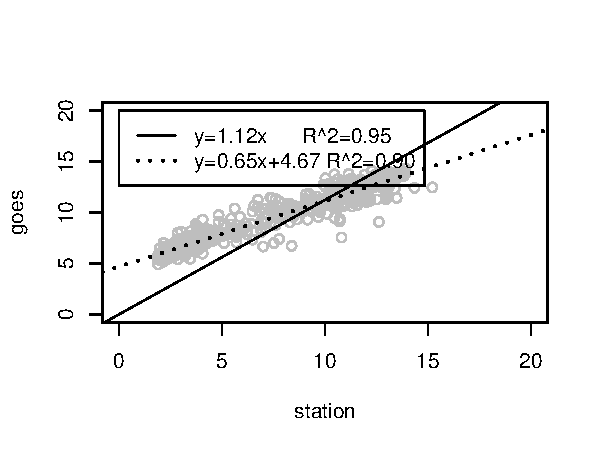
\includegraphics[width=1\textwidth]{winter_fog_Rs_R.pdf}
%\end{frame}

\end{document}



